\section{Passive Elemente}

\begin{longtable}{|>{\bfseries}p{3cm}|c|p{10cm}|}
    \hline
    Widerstand
    & 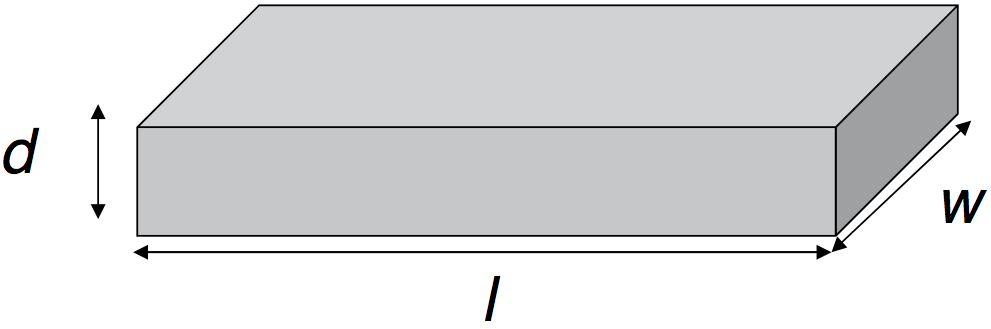
\includegraphics[width=4cm, valign=t]{pictures/widerstand.png}
    & {$R=\rho \cdot \frac{l}{w\cdot d}$ \qquad $\rho$: Spezifischer Widerstand
      }
    \\ \hdashline
    {PTC (Kaltleiter)\newline
     am Beispiel\newline
     PT1000
    }
    &
    & {Berechnung des Widerstandes für Temp $>$ 0°C:\newline
       $R = R_0 \cdot (1 + \alpha t + \beta t^2)$\newline
       Berechnung des Widerstandes für Temp $<$ 0°C:\newline
       \begin{align*}
           R &= R_0 \cdot [1 + \alpha t + \beta t^2 + \gamma \cdot (t - 100 ^\circ C)\cdot t^3]\\
           \alpha &= 3.9083 \cdot 10^{-3} 1/ ^\circ C\\
           \beta &= -5.775 \cdot 10^{-7} 1/ ^\circ C^2\\
           \gamma &= -4.183 \cdot 10^{-12} 1/ ^\circ C^4
       \end{align*}
      }
    \\ \hdashline
    {NTC\newline
     (Heissleiter)
    }
    &
    & {$R_T = R_R \cdot e^{B\cdot\left( \frac{1}{T} - \frac{1}{T_R}\right) }$\newline
       $\mathrm{R_T}$: NTC-Widerstand bei Temperatur T in Kelvin\newline
       $\mathrm{R_R}$: NTC-Widerstand bei definierter Temperatur $\mathrm{T_R}$ in Kelvin\newline
      }
    
    \\ \hline
    % ----------------------------------------------------------------------------------------------------
    Kondensator
    & 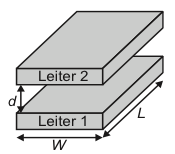
\includegraphics[width=4cm, valign=t]{pictures/kapazitaetswert.png}
    & {$C=\varepsilon_{r}\cdot \varepsilon_{0}\cdot \frac{W\cdot L}{d}=\varepsilon_{r}\cdot \varepsilon_{0}\cdot \frac{A}{d}$ \qquad $\varepsilon_{0}= 8.85 pF/m$\newline
       \newline
       \begin{align*}
           \intertext{\textbf{Ladevorgang:}}
           u_{\mathrm{C}} (t) &= U_0 \cdot \left( 1 - e^{- \frac{t}{\tau}}\right)  = U_0 \cdot \left( 1 - e^{- \frac{t}{R \cdot C}}\right)\\
           i_{\mathrm{C}} (t) &= \frac{U_0}{R} \cdot e^{- \frac{t}{\tau}} = I_0 \cdot e^{- \frac{t}{R \cdot C}}\\
           \intertext{\textbf{Entladevorgang:}}
           u_{\mathrm{C}} (t) &= U_0 \cdot e^{- \frac{t}{\tau}} = U_0 \cdot e^{-\frac{t}{R \cdot C}}\\
           i_{\mathrm{C}} (t) &= -\frac{U_0}{R} \cdot e^{- \frac{t}{\tau}} = - I_0 \cdot e^{-\frac{t}{R \cdot C}}
       \end{align*} \newline
      \textbf{Dielektrizitätsklassen:}\newline
      \begin{tabular}{|p{2cm}|l|p{2cm}|p{2cm}|}
        \hline
          \textbf{Code} &
          C0G, NP0 &
          X5R, X7R & 
          Y5U, Z5U \\
        \hline
          \textbf{Tempera- turbereich} &
          $-55\ldots125^{\circ}C$ &
          X5R: $-55\ldots85^{\circ}C$ \newline
          X7R: $-55\ldots125^{\circ}C$ &
          Y5U: $-30\ldots85^{\circ}C$ \newline
          Z5U: $10\ldots85^{\circ}C$ \\
        \hline
          \textbf{Kapazität- sänderung über Temperaturbereich} &
          $0 \pm 30ppm$ &
          $\pm 15 \%$ &
          $\pm 40 \%$ \\
        \hline
          \textbf{max. Kapazität im 1206 Gehäuse} &
          $0.1\mu F/25V$ &
          X5R: $100\mu F/6.3V$ \newline
          X7R: $10\mu F/16V$ &
          $22\mu F/16V$ \\
        \hline
      \end{tabular}
      }
    \\ \hline
    % ----------------------------------------------------------------------------------------------------
    Induktivität
    & 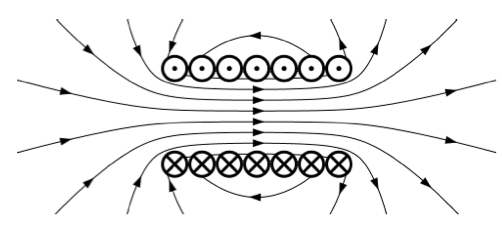
\includegraphics[width=4cm, valign=t]{pictures/induktivitaet.png}
    & {\begin{align*}
           L &=N^2\cdot\frac{\mu_{0}\mu_{r}A}{2\pi r} \qquad \text{Ringspule} \\
           L &=N^2\cdot\frac{\mu_{0}\mu_{r}A}{l} \qquad \text{Zylinderspule} \\
           L &=\frac{N\cdot\Phi}{I} \qquad \qquad u_{i} =-N\cdot\frac{d\Phi}{dt}\\
           \intertext{\textbf{Ladevorgang:}}
           i_{\mathrm{L}} (t) &= I_0 \cdot \left( 1 - e^{-\frac{t}{\tau}}\right) = \frac{U_0}{R} \cdot \left( 1 -e^{-t\cdot \frac{R}{L}}\right) \\
            u_{\mathrm{L}} (t) &= \hat u \cdot e^{-\frac{t}{\tau}} = \hat u \cdot e^{-t \cdot\frac{R}{L}}\\
            \intertext{\textbf{Entladevorgang:}}
            i_{\mathrm{L}} (t) &= I_0 \cdot e^{- \frac{t}{\tau}} = \frac{U_0}{R} \cdot e^{- t \cdot\frac{R}{L}}\\
            u_{\mathrm{L}} (t) &= - \hat u \cdot e^{- \frac{t}{\tau}} = - \hat u \cdot e^{- t \cdot\frac{R}{L}}
       \end{align*}
      }
    \\ \hline
    \multicolumn{2}{|c}{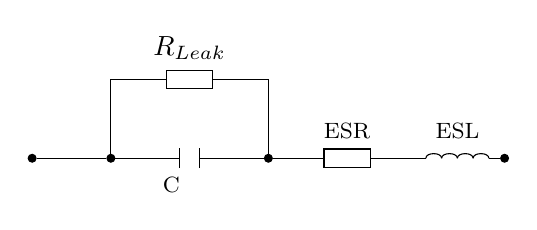
\begin{tikzpicture}

  \node (dot) at (1,1) [draw,circle,inner sep=1,fill]{};
  \node (dot2) at (2,1) [draw,circle,inner sep=1,fill]{};

  \node (c) at (3,1) [rectangle]{};
  \node (rleak) at (3,2)[draw,rectangle]{$~~~$};
  \node (dot3) at (4,1) [draw,circle,inner sep=1,fill]{};
  \node (esr) at (5,1)[draw,rectangle]{$~~~$};
  \coordinate (eslstart) at (6,1);
  \coordinate (eslend) at (6.8,1);
  \node (esl) at (6,1)[rectangle]{};
  \node (dot4) at (7,1) [draw,circle,inner sep=1,fill]{};

  \draw (dot) -- (dot2) -- (c) -- (dot3) -- (esr) -- (eslstart) (eslend) -- (dot4);
  \draw (dot2) |- (rleak) -| (dot3);

  \draw (c.south west) -- (c.north west);
  \draw (c.south east) -- (c.north east);

 \begin{scope}[out=90,in=90]
   \foreach \x in {0,0.2,0.4,0.6}
      \draw (eslstart)++(\x,0) to ++(0.2,0);
 \end{scope}

 \draw (rleak.north) node[above]{$R_{Leak}$};
 \draw (esr.north) node[above]{\footnotesize ESR};
 \draw (esl.north) node[above right]{\footnotesize ESL};
 \draw (c.south) node[below left]{\footnotesize C};


\end{tikzpicture}
}
    & \multicolumn{1}{|c|}{\begin{tikzpicture}

  \node (dot) at (1,1) [draw,circle,inner sep=1,fill]{};
  \node (dot2) at (2,1) [draw,circle,inner sep=1,fill]{};

  \node (c) at (3.5,2) [rectangle]{};
  \node (l) at (3,1)[rectangle]{};
  \coordinate (lstart) at (2.6,1);
  \coordinate (lend) at (3.4,1);
  \node (rcu) at (4,1)[draw,rectangle]{$~~~$};
  \node (dot3) at (5,1) [draw,circle,inner sep=1,fill]{};
  \node (dot4) at (6,1) [draw,circle,inner sep=1,fill]{};

  \draw (dot) -- (dot2) -- (lstart) (lend) --(rcu)  -- (dot3)  -- (dot4);
  \draw (dot2) |- (c) -| (dot3);

  \draw (c.south west) -- (c.north west);
  \draw (c.south east) -- (c.north east);

 \begin{scope}[out=90,in=90]
   \foreach \x in {0,0.2,0.4,0.6}
      \draw (lstart)++(\x,0) to ++(0.2,0);
 \end{scope}

 \draw (rcu.south) node[below]{\footnotesize $R_{Cu}$};
 \draw (l.south) node[below]{\footnotesize L};
 \draw (c.north) node[above]{\footnotesize $C_p$};

\end{tikzpicture}
}\\
    \multicolumn{2}{|c}{Ersatzschaltung Kondensator}
    & \multicolumn{1}{|c|}{Ersatzschaltung Spule} \\
    \multicolumn{2}{|c}{}
    & \multicolumn{1}{|c|}{Bestimmung von $C_p$: letzten Punkt der Kurve nehmen, $Z_f=\frac{1}{2*\varPi*f*C_p}$}
    \\ \hline
\end{longtable}


